% Report Template in LaTeX

\documentclass[12pt]{article}

% Packages
\usepackage{graphicx} % For including images
\usepackage{geometry} % For adjusting page margins
\usepackage{titlesec} % For customizing section titles
\usepackage{setspace} % For line spacing
\usepackage{hyperref} % For hyperlinks
\usepackage{amsmath} % For mathematical equations
\usepackage{amsfonts} % For mathematical fonts
\usepackage{amssymb} % For mathematical symbols
\usepackage{fancyhdr} % For custom headers and footers
\usepackage{enumitem} % Add this to the preamble
\usepackage{booktabs}


% Page layout
\geometry{a4paper, margin=1in} 
\setlength{\parindent}{0pt}
\setlength{\parskip}{1em}

% Line spacing
\onehalfspacing

% Section title formatting
% Customize section numbers for document but not table of contents
\renewcommand{\thesection}{\arabic{section}}
\titleformat{\section}{\normalfont\Large\bfseries}{Problem \arabic{section}}{1em}{}
\renewcommand{\thesubsection}{\thesection\alph{subsection}}
\titleformat{\subsection}{\normalfont\large\bfseries}{\thesubsection}{1em}{}

% Header and footer
\pagestyle{fancy}
\fancyhf{}
\fancyhead[L]{\leftmark}
\fancyhead[R]{\thepage}
\renewcommand{\headrulewidth}{0.4pt}

% Title Page
\title{\textbf{Report Title}}
\author{Author Name \\ Department \\ Institution}
\date{\today}
\begin{document}

% Title Page
\begin{titlepage}
    \centering
    \vspace*{2cm}
    {\Huge\bfseries HW1: Regression, Cross-Validation, and Regularization\par}
    \vspace{1.5cm}
    {\Large\itshape Vedant Modi\par}
    \vspace{0.5cm}
    {\large COMP135: Introduction to Machine Learning\par}
    {\large Spring 2025, Tufts University \par}
    \vspace{2cm}
    {\large \today\par}
    \vfill
\end{titlepage}

% Table of Contents
% \tableofcontents
\newpage

% % Abstract
% \section*{Abstract}
% \addcontentsline{toc}{section}{Abstract} % Add abstract to table of contents
% This is the abstract of the report. It provides a brief summary of the contents, including the purpose, methods, results, and conclusions. Keep it concise and to the point.

% \newpage

% Introduction
\section{}
\subsection{Short answer}
The weight coefficient values (to 2 decimal places) for each of the $F$
 features of the degree = 1 model are as follows
\begin{verbatim}
    -10.43 : x0
    -18.23 : x1
     -1.15 : x2
      0.58 : x3
   where 
   x0 = horsepower
   x1 = weight
   x2 = cylinders
   x3 = displacement
\end{verbatim}

\subsection{Short answer}
Intuitively, the heavier the engine, the \textit{less} efficient the vehicle is
bound to be. This is because the engine needs to expel more force to propel a
larger weight. This would result in a negative correlation between weight and
the mpg of the vehicle.

On the other hand, a higher engine displacement means that there is more volume
of air being moved through the engine. So, one might think that the mpg is
higher with a higher engine displacement. However, we also know that a larger
engine would have a higher engine displacement. A larger engine necessitates a heavier
engine, and thus a diminishing mpg for the vehicle. 

In other words, the relationship could go both ways, a higher displacement on a
small enough engine would cause a higher mpg. But, a higher displacement on an
engine that is too large, would cause a lower mpg. For this reason, the
magnitude of the weight is very low.
\subsection{Short answer}
The magnitudes of the weights in degree 4 are much higher than those in lower
degrees (like degree 1, or degree 2). This is likely because of the idea we
discussed in lecture, where the degree 4 polynomial will make large adjustments
to try to hit all the training points, but perform worse in validation tests. 

\begin{figure}[htbp!]
    \centering
    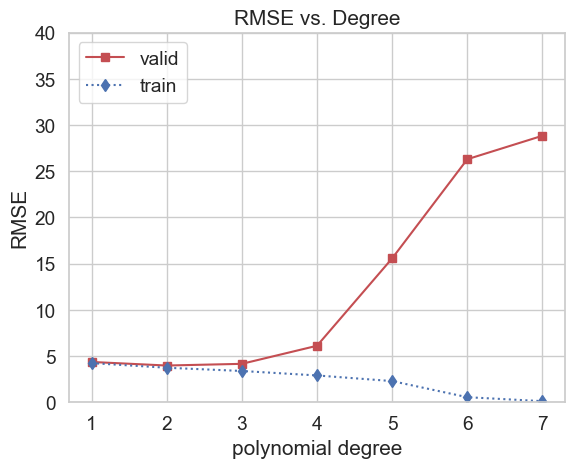
\includegraphics[width=0.5\textwidth]{1c.png}
    \caption{Chosen degree is 2}

    \begin{enumerate}[label=(\roman*)]
        \item I have chosen degree 2 since this minimizes the distance between
        RMSE of training and validation sets. At the same time, the validation
        error starts to increase at degrees higher than 2. This implies that
        for models with degree $> 2$, there might be overfitting. That is, the
        model may find difficulty in generalizing on ``never-seen-before''
        data. 
        
        On the other hand, I selected a degree 2 polynomial over a degree
        1 polynomial as minimized the effect of ``underfitting'' as well. That
        is, there are enough features that are being added such that both the
        training and validation data report lower errors. 

        \item Overfitting can be seen in higher degrees of the polynomial.
        (degrees 5, 6, 7) 
        
        We can tell that there is overfitting because the
        large differential between validation error and training error. We can
        tell this is overfitting because although training error is low (i.e.
        the model can predict the response for the training examples with great
        performance), we can see the validation error is very high. A very high
        validation error means that the model does not generalize well. This
        means that on new data, that the model is not trained on, we see worse
        performance (higher error). 
    \end{enumerate}
\end{figure}

\subsection{Short answer}
Training error has a lower rate of increase going from degree 6 to degree 7, as
compared to degree 5 to degree 6. This can be thought of as the model
``overfitting'', which is seen at higher degrees of regression, as discussed in
day03 and day04. 

\subsection{Short answer}

\renewcommand{\thefigure}{1.1}
\begin{figure}[htbp]
    \centering
    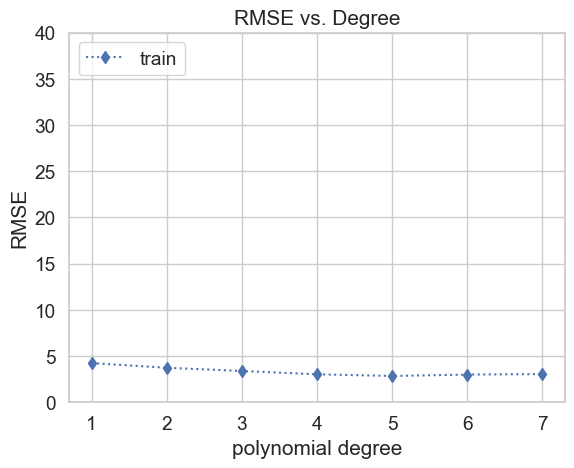
\includegraphics[width=0.5\textwidth]{1e.png}
    \caption{Lower training error compared to Figure 1}
    \label{fig:1e}
\end{figure}
\renewcommand{\thefigure}{\arabic{figure}} 
\setcounter{figure}{1}

Train error increases slightly at higher degrees without the prescence of
\verb|MinMaxScaling|. This is because with \verb|MinMaxScaling|, we produce
weights of lesser magnitude, relative to without \verb|MinMaxScaling|. We've
seen before that with higher magnitude weights, we are prone to overfitting the
model, as the coefficients will be very close to the training data, and perform
very well on the training data. This leads to a lower error in the training
data, which is what we see in \autoref{fig:1e}. 

It's useful to scale raw input features to be within the range $[0,1]$ as it
brings the magnitudes of weights down. This way, we avoid overfitting (at
higher degrees) as it
occurred in the aforementioned example. 

\pagebreak

\section{}

\begin{figure}[htbp]
    \centering
    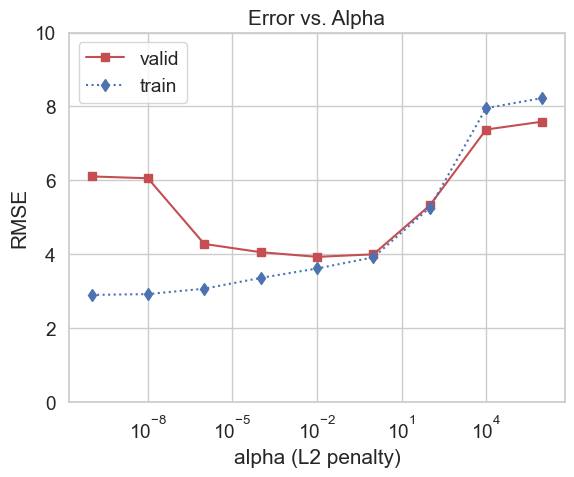
\includegraphics[width=0.5\textwidth]{2a.png}
    \caption{Error vs. Alpha}
    \label{fig:2a}

    \begin{enumerate}[label=(\roman*)]
        \item As $\alpha$ increases, we start seeing a decrease in validation error. Then,
        at some minima, the validation error starts to increase again. On the
        other hand, training error is always increasing with higher $\alpha$.
        \item We should choose the $\alpha$ that leads to the least validation 
        error to perform best on new data. This is because the model has not
        been fitted with this data, so does not know the responses of these
        examples. So, we get a more true sense of how the model will perform
        out in the ``real world''. So, I would choose $\alpha = 1 \times 10^{-2}$.
    \end{enumerate}
\end{figure}

\subsection{Short answer}
% Inspect the learned weight parameters of your chosen degree-4 model.
% What do you notice about the relative magnitudes compared to the degree-4 model from Problem 1?
In the degree-4 model of Problem 1, the magnitudes of the weights are much
larger than the chosen degree-4 model in this problem. This is likely because
the L2 regression which we are now using has a term that penalizes large terms.
So, larger magnitudes will now be lesser than those derived from a degree-4
regression without any penalization. 

\subsection{Short answer}

% What numerical value of α̂  would this strategy favor? (Hint: you aren't
% limited to the grid in 2A). 
% Why is this problematic if your goal is to generalize to new data well?
To minimize the formula given, we would choose an $\alpha$ that is small as
possible (i.e. $\alpha = 0$) since we want to minimize the whole expression,
and any $\alpha > 0$ would increase the value of the expression. 

For an $\alpha = 0$, we recover the unpenalized regression, which would lead to
the same high degree model that we saw overfitting in. With overfitting, we
have a tendency to not generalize new data well, which would eliminate the
purpose of penalties. 
\pagebreak
\section{}
\setcounter{table}{2}
\begin{table}[h]
    \centering
    \begin{tabular}{lllr}
        \toprule
         & name & hypers & testRMSE \\
        \midrule
        0 & predict mean of train ys &  & 8.231074 \\
        1 & LR deg=best-on-val & deg: 2 & 3.991503 \\
        2 & ridgeLR deg=4 alph=best-on-val & alph: 1e-06 & 3.877668 \\
        3 & ridgeLR deg=best-on-CV alph=best-on-CV & deg: 7 alph: 0.1 & 3.816827 \\
        \bottomrule
        \end{tabular}
    \caption{Various RMSE's from regressors}

    \begin{enumerate}[label=(\roman*)]
        \item Problem 3's model sees better performance than Problem 2's model
        since we were able to select between the best degree and $\alpha$ in
        Problem 3. In Problem 2, we only selected the best $\alpha$, and fixed
        a degree, 4. Note that in Problem 3, we chose a higher degree, 7.
        Therefore, we likely saw some underfitting occur in Problem 2's model,
        and Problem 3 improved that by increasing model complexity. At the same
        time however, there might have been some decreased generalization. For
        this reason, we included an $\alpha$ parameter to decrease the
        magnitudes of the weights. This improves the generalization of the
        model in Problem 3, outperforming Problem 2's model.

        We also have used cross validation when determining the model in
        Problem 3. This improves generalization as well, since we train using
        different sets of data, and reduce bias derived from using a specific
        set of training data. That is, all data gets a chance to be trained on,
        and we choose the set of data that has the best performance on the
        validation set. This way, we can observe more data to train the model,
        and improving generalization. For this reason, Problem 3's model also
        performs better than Problem 2.

        \item We can't just select a degree and an $\alpha$ to minimize test
        set error, since we could potentially underfit the model, and actually
        end up hurting the generalization. We need to also verify that the
        training error is low enough, and not decreasing with an increased complexity.
        % high magn
        
    \end{enumerate}
    
\end{table}




\end{document}